\documentclass[11pt]{article}

% load some asm stuff -
\usepackage{amsthm}
\usepackage{amssymb,amsmath}
\usepackage{mathtools}
%\usepackage{palatino,lettrine}
\usepackage{fancyhdr}
\usepackage{epsfig}
\usepackage[round,comma,sort]{natbib}
\usepackage{simplemargins}
\usepackage{setspace}
\usepackage[margin=0pt,font=small,labelfont=bf]{caption}

\bibliographystyle{plos2009}

% Set the size
%\textwidth = 6.75 in
%\textheight = 9.75 in
%\oddsidemargin = 0.0 in
%\evensidemargin = 0.0 in
%\topmargin = 0.01 in
%\headheight = 0.0 in
%\headsep = 0.25 in
%\parskip = 0.15in
\doublespace

\setallmargins{1in}

\newtheorem{example}{Example}[section]
\newtheorem{thm}{Theorem}[section]
\newtheorem{property}{Property}[section]

\theoremstyle{definition}
\newtheorem{defn}[thm]{Definition}

\makeatletter
\renewcommand\subsection{\@startsection
	{subsection}{2}{0mm}
	{-0.05in}
	{-0.5\baselineskip}
	{\normalfont\normalsize\bfseries}}
\renewcommand\subsubsection{\@startsection
	{subsubsection}{2}{0mm}
	{-0.05in}
	{-0.5\baselineskip}
	{\normalfont\normalsize\itshape}}
\renewcommand\paragraph{\@startsection
	{paragraph}{2}{0mm}
	{-0.05in}
	{-0.5\baselineskip}
	{\normalfont\normalsize\itshape}}
\makeatother
\linespread{1.2}

\fancypagestyle{proposal}{\fancyhf{}%
	\fancyhead[RO,LE]{\thepage}%
	\fancyhead[LO,RE]{ChE 525 Metabolic Flux Analysis (MFA)}%
	\renewcommand\headrulewidth{1pt}}
\pagestyle{proposal}

% Single space'd bib -
\setlength\bibsep{0pt}

\renewcommand{\rmdefault}{phv}\renewcommand{\sfdefault}{phv}

%\newboxedtheorem[boxcolor=black, background=gray!5,titlebackground=orange!20,titleboxcolor = black]{color_box_example}{Example}{test}

% Change the number format in the ref list -
\renewcommand{\bibnumfmt}[1]{#1.}

% Change Figure to Fig.
\renewcommand{\figurename}{Fig.}

%Joycelyn Chan, Joshua Lequieu, Michael Paull, Chidanand Balaji, Ryan Tasseff
%Our derivation follows closely the earlier development of Fredrickson \citep{Fredrickson:1976fk}.

% Begin ...
\begin{document}

%\begin{titlepage}
{\par\centering\textbf{\Large Intracellular Metabolic Networks and Metabolic Flux Analysis}}
\vspace{0.2in}
{\par \centering \large{Jeffrey D. Varner$^{*}$}}
\vspace{0.05in}
{\par \centering \large{School of Chemical Engineering$^{*}$}}
{\par \centering \large{Purdue University, West Lafayette IN 47907}}
\vspace{0.1in}
{\par \centering \small{Copyright \copyright\ Jeffrey Varner 2016. All Rights Reserved.}}\\

%\end{titlepage}
\date{}
\thispagestyle{empty}

\setcounter{page}{1}

%material and energy balances around the different processes cells do. For example, understanding how the abundance of raw materials in a bioreactor influences
%cell growth, or the production of valuable protein or small molecule products requires a materials balances around the major components of the system.
%The production of valuable small molecule or protein products requires large connected intracellular reaction networks that produce or consume energy.
%Thus, to understand the operation of biochemical systems and ultimately to manipulate them for societal gain,

%We developed material balances for nutrients, products and cells for batch, fed-batch and continuous stirred tank bioreactors.
%We also considered the \textit{best} way to operate bioreactors, for example, to maximize the amount of the product or
%the rate of product production in a given time period by varying process parameters, such as volumetric flow rate.
%However, we have not considered the problem of changing the \textit{intracellular} operation of cells.

\section*{Introduction}
Cells operate vast interconnected biochemical \textit{networks} to process starting materials such as sugars into valuable products of interest, waste products and eventually more cells.
Previously, we derived a material balance governing the specific intracellular concentration of the $j^{th}$ metabolite $x_{j}$ [mmol/gdw] in an arbitrary metabolic network:
\begin{equation}\label{eqn-final-mass-balance}
	\frac{dx_{j}}{dt} = \left(\displaystyle\sum_{r}^{\mathcal{R}}\sigma_{jr}v_{r} + \displaystyle\sum_{k}^{\mathcal{T}}\tau_{jk}q_{k}\right) - \mu x_{j}
	\qquad{j=1,2,\hdots,\mathcal{M}}
\end{equation}or in matrix-vector:
\begin{equation}
	\frac{d\mathbf{x}}{dt} = \mathbf{S}\mathbf{v} + \mathbf{T}\mathbf{q} -\mu\mathbf{x}
\end{equation}where $\mathbf{x}$ denotes the species abundance vector ($\mathcal{M}\times{1}$), $\mathbf{S}$ denotes the stoichiometric matrix ($\mathcal{M}\times{\mathcal{R}}$),
and $\mathbf{T}$ ($\mathcal{M}\times{\mathcal{T}}$) denotes the transport (or exchange) matrix.
Given these balance equations, we could estimate the steady-state flux (specific reaction rates $\mathbf{v}, \mathbf{q}$) through the network using flux balance analysis:
\begin{equation}
\begin{multlined}
	\qquad \qquad \qquad \max_{\boldsymbol{v}}{} \! \left( v_{obj} = \mathbf{c}^T \boldsymbol{v} \right) \\
	\mathrm{Subject \; to:}
	 \; \; \mathbf{S}\mathbf{v}=-\mathbf{Tq} \\
\alpha_i \leq v_i \leq \beta_i  \qquad
\end{multlined}
\end{equation}
where $\mathbf{c}^{T}$ is the \textit{objective selection vector} and $\mathbf{S}$ and $\mathbf{T}$ denote the stoichiometric and transport arrays for both intracellular and extracellular metabolites (rows)
for unmeasured and measured fluxes (columns).
However, flux balance analysis is not the only technique that can be used to estimate intracellular metabolic flux.
Metabolic flux analysis (MFA) is another widely used approach that relies on linear algebra (and not linear programming) to compute the unknown metabolic flux vector.

\subsection*{Metabolic Flux Analysis (MFA).}
Similar to flux balance analysis, metabolic flux analysis relies upon a pseudo steady-state assumption to reduce the intracellular material balance equations to a system of algebraic equations:
\begin{equation}\label{eqn-mfa-ss-w-metabolites}
	\mathbf{S}\mathbf{v} + \mathbf{T}\mathbf{q} -\mu\mathbf{x}^{*}\simeq\mathbf{0}
\end{equation}where $\mathbf{x}^{*}$ denotes the steady-state species abundance vector.
Eqn \eqref{eqn-mfa-ss-w-metabolites} has two sets of unknowns, the states and the fluxes.
Without direct experimental measurements of the intracellular state of the cell, we have way of knowing $\mathbf{x}^{*}$.
Moreover, we know the dilution due to growth terms ($\mu\mathbf{x}^{*}$) are small compared to the metabolic flux terms.
Thus, we typically drop the dilution terms to arrive at:
\begin{equation}\label{eqn-mfa-ss-wno-metabolites}
	\mathbf{S}\mathbf{v} + \mathbf{T}\mathbf{q} \simeq\mathbf{0}
\end{equation}Eqn \eqref{eqn-mfa-ss-wno-metabolites} are $\mathcal{M}$ algebraic equations in the unknown intracellular fluxes $v_{1},\hdots,v_{\mathcal{R}}$ and transport fluxes
$q_{1},\hdots,q_{\mathcal{T}}$. Typically, $\mathcal{M}<\mathcal{R}+\mathcal{T}$ which means that no unique flux solution can be found.
However, we can potentially measure some of the transport fluxes that carry material into and from the cells. Denote the subset of \emph{measured} fluxes
as $\vartheta_{m}$ ($\mathcal{E}\times{1}$ column vector), and all other unmeasured fluxes as $\vartheta_{u}$ ($\mathcal{U}\times{1}$ column vector).
We can then redefine the stoichiometric balances as:
\begin{equation}\label{eqn-mfa-ss-wno-metabolites-split}
	\mathbf{\Sigma}\vartheta_{u} + \mathbf{\Phi}\vartheta_{m} \simeq\mathbf{0}
\end{equation}where $\mathbf{\Phi}$ contains the columns corresponding to the measured fluxes ($\mathcal{M}\times\mathcal{E}$), and $\mathbf{\Sigma}$ contains
the columns corresponding to \emph{unmeasured} fluxes ($\mathcal{M}\times\mathcal{U}$).
Eqn \eqref{eqn-mfa-ss-wno-metabolites-split} can be solved for the \emph{unmeasured} fluxes $\vartheta_{u}$:
\begin{equation}
	\vartheta_{u}\simeq-\mathbf{\Sigma}^{\#}\mathbf{\Phi}\vartheta_{m}
\end{equation}where $\mathbf{\Sigma}^{\#}$ is a $\mathcal{U}\times\mathcal{M}$ \emph{generalized} matrix inverse.
The functional form of the generalized inverse depends upon the shape and properties of the unmeasured stoichiometric array $\mathbf{\Sigma}$.

The matrix $\mathbf{\Sigma}^{\#}$ is the generalized inverse of the stoichiometric matrix corresponding to the \emph{unmeasured} fluxes.
The form of $\mathbf{\Sigma}^{\#}$ depends upon the shape and the \emph{rank} of $\mathbf{\Sigma}$.
The definition of the $\mathbf{\Sigma}$ and $\mathbf{\Phi}$ arrays influences our ability to solve the intracellular material balances. The structure of these arrays
is controlled practically by which fluxes are measured. Measurement selection is influenced by several factors, technical concerns regarding the measurement
technology, the cost of measurements as well as the time required to make measurements.

\begin{itemize}

\item{$\mathcal{M}>\mathcal{U}$: \textbf{Overdetermined system of equations.}
Overdetermined systems are characterized by more equations than unknowns and have no single \emph{regular} solution, in other
words, no single solution that simultaneously satisfies all material balance equations.
The problem of determining the solution to an overdetermined system can be recast as the least-squares problem:
\begin{equation}\label{eq-ose}
\min_{\mathbf{\vartheta_{u}}}\bigl(\mathbf{\Sigma\vartheta_{u}}-\mathbf{b}\bigr)^{T}\bigl(\mathbf{\Sigma\vartheta_{u}}-\mathbf{b}\bigr)
\end{equation}where
\begin{equation}
\mathbf{b}\equiv-\mathbf{\Phi\vartheta_{m}}\left(t\right)
\end{equation}
Equation \eqref{eq-ose} can be solved analytically by using standard tools from calculus to yield the solution:
\begin{equation}\label{eq-right}
\mathbf{\vartheta_{u}}=\left(\mathbf{\Sigma^{T}\Sigma}\right)^{-1}\mathbf{\Sigma^{T}b}
\end{equation}In this case the quantity $\mathbf{\Sigma}^{\#}$ is given by:
\begin{equation}
\mathbf{\Sigma}^{\#} = \mathbf{\Sigma^{L}}\equiv\left(\mathbf{\Sigma^{T}\Sigma}\right)^{-1}\mathbf{\Sigma^{T}}
\end{equation}denotes a \emph{left} inverse (sometimes called the left Moore-Penrose inverse, left generalized inverse or pseudo inverse).
For the least-squares solution Equation
\eqref{eq-right} to exist, the condition
\begin{equation}
\det\mathbf{\Sigma^{T}\Sigma}\neq{0}
\end{equation}must be satisfied.}

\item{$\mathcal{M}<\mathcal{U}$: \textbf{Underdetermined system of equations.}
Underdetermined systems are characterized by $\infty$-solutions as $n$ unknowns can be written in terms of the remaining $m-n$
unknowns which in the general case take on arbitrary values. The solution of an underdetermined system of LAEs can be posed
as a constrained least-squares minimization problem of the form:
\begin{equation}\label{eq-under}
\min_{\mathbf{u}}\frac{1}{2}\mathbf{\vartheta_{u}}^{T}\mathbf{\vartheta_{u}}
\end{equation}subject to:
\begin{equation}
\mathbf{\Sigma\vartheta_{u}}=\mathbf{b}
\end{equation}where
\begin{equation}
\mathbf{b}\equiv-\mathbf{\Phi\vartheta_{m}}\left(t\right)
\end{equation}
Problem \eqref{eq-under} can also be solved analytically using standard tools from calculus to yield the solution:
\begin{equation}
\mathbf{\vartheta_{u}}=\mathbf{\Sigma}^{T}\left(\mathbf{\Sigma\Sigma}^{T}\right)^{-1}\mathbf{b}
\end{equation}
The quantity
\begin{equation}\label{eq-left}
\mathbf{\Sigma}^{\#} = \mathbf{\Sigma^{R}}\equiv\mathbf{\Sigma^{T}}\left(\mathbf{\Sigma\Sigma^{T}}\right)^{-1}
\end{equation}denotes a \emph{right} inverse (sometimes called the right Moore-Penrose inverse, right generalized inverse or pseudo inverse).
For the least-squares solution Equation
\eqref{eq-left} to exist, the condition
\begin{equation}
\det\mathbf{\Sigma\Sigma^{T}}\neq{0}
\end{equation}must be satisfied.}

\item{$\mathcal{M}=\mathcal{U}$: \textbf{Square system of equations.}
When the number of equations equals the number of unknowns the system is said to be \emph{square}. Square systems can be
solved by several different techniques, including directly determining the matrix inverse $\mathbf{\Sigma}^{-1}$, i.e.,
\begin{equation}\label{eq-square-soln}
\mathbf{\vartheta_{u}}=-\mathbf{\Sigma}^{-1}\mathbf{\Phi\vartheta_{m}}\left(t\right)
\end{equation}Solution \eqref{eq-square-soln} exists as along as:
\begin{equation}
\det\left(\mathbf{\Sigma}\right)\neq{0}
\end{equation}
However, the direct computation of the inverse for square systems is \emph{very} computationally expensive. Thus, in practice
other techniques, such as Gauss Elimination (GE), Gauss Jordan Elimination (GJE) or iterative techniques (ITs) are used to calculate the flux
vector $\mathbf{\vartheta_{u}}$.}
\end{itemize}

An alternative to computing the determinant to check the existence of the matrix inverse, is to compute the rank.
The rank of the $N\times{M}$ matrix $\mathbf{A}$ given by:
\begin{equation}
	rank\left(\mathbf{A}\right)\leq\min\left(N,M\right)
\end{equation}is a measure of the independent information contained in the rows and columns of a matrix.
Arrays with linearly independent rows and columns have full rank, while arrays with linearly dependent components are not full rank.
For a determinant to be non-zero, an array has to be full rank. Performing a rank test is more efficient that computing the determinant of a matrix, especially for large non-square matrices.


\begin{figure*}[h!]\centering
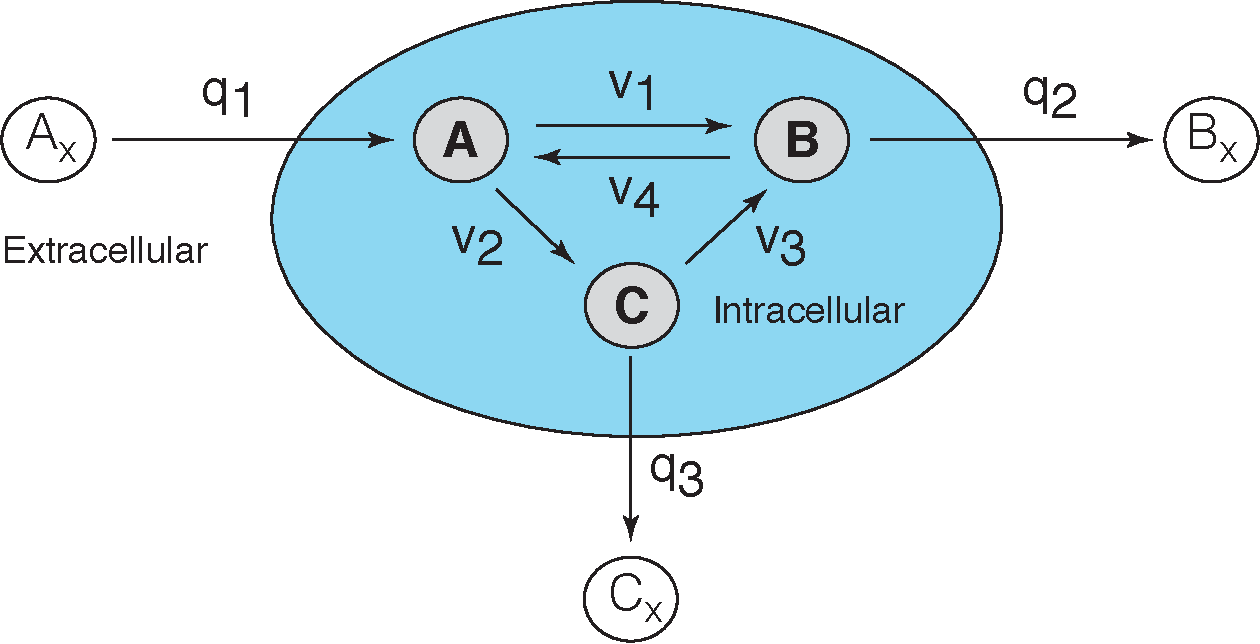
\psfig{file=figs/Simple-network-example.pdf,width=0.8\textwidth}
\caption{Schematic of simple metabolic reaction network. This system has a total of six metabolites and seven reactions.
The intracellular metabolites (metabolites $A,B$ and $C$) are often treated as balanced (no accumulation) while the extracellular metabolites ($A_{x},B_{x}$ and $C_{x}$) are not balanced (can accumulate).
The blue-oval denotes the cell boundaries, where $q_{j}$ denotes flux across these boundaries ([mmol/gdw-hr]) and $v_{k}$ denotes the intracellular fluxes.}\label{fig-system}
\end{figure*}

\subsubsection*{Example: Proof of concept MFA with a toy network.}
Estimate the intracellular fluxes for the simple reaction network shown in Fig. \eqref{fig-system} using metabolic flux analysis (MFA).
Assuming we measured all three transport fluxes, the stoichiometric and transport arrays for this network are given by:
\begin{equation}
\mathbf{\Sigma} =
\begin{bmatrix}
	-1 & -1 & 0 & 1 \\
	1 & 0 & 1 & -1 \\
	0 & 1 & -1 & 0 \\
\end{bmatrix}
\end{equation} and
\begin{equation}
	\mathbf{\Phi} =
	\begin{bmatrix}
		1 & 0 & 0 \\
		0 & -1 & 0 \\
		0 & 0 & -1 \\
	\end{bmatrix}
\end{equation}
The stoichiometric matrix $\mathbf{\Sigma}$ is not square nor does it have full rank $rank\left(\mathbf{\Sigma}\right)$ = 2.
Thus, even the pseudo inverse is not defined for this set of measured fluxes, suggesting we need to change our experimental design.
If we measure only $q_{1}$ and $q_{2}$, the stoichiometric and transport arrays become:
\begin{equation}
\mathbf{\Sigma} =
\begin{bmatrix}
	-1 & -1 & 0 & 1 & 0 \\
	1 & 0 & 1 & -1 & 0 \\
	0 & 1 & -1 & 0 & -1 \\
\end{bmatrix}
\end{equation} and
\begin{equation}
	\mathbf{\Phi} =
	\begin{bmatrix}
		1 & 0 \\
		0 & -1 \\
		0 & 0 \\
	\end{bmatrix}
\end{equation}which has full rank $rank\left(\mathbf{\Sigma}\right)$ = 3.
We can compute a right inverse and solve for $\vartheta_{u} = \left(v_{1},v_{2},v_{3},q_{3}\right)$.
If we assume $q_{1} = 1.0$ and $q_{2} = 0.5$, the flux solution is shown in Fig. \eqref{fig-bad-flux-solution}.

\begin{figure*}[h!]\centering
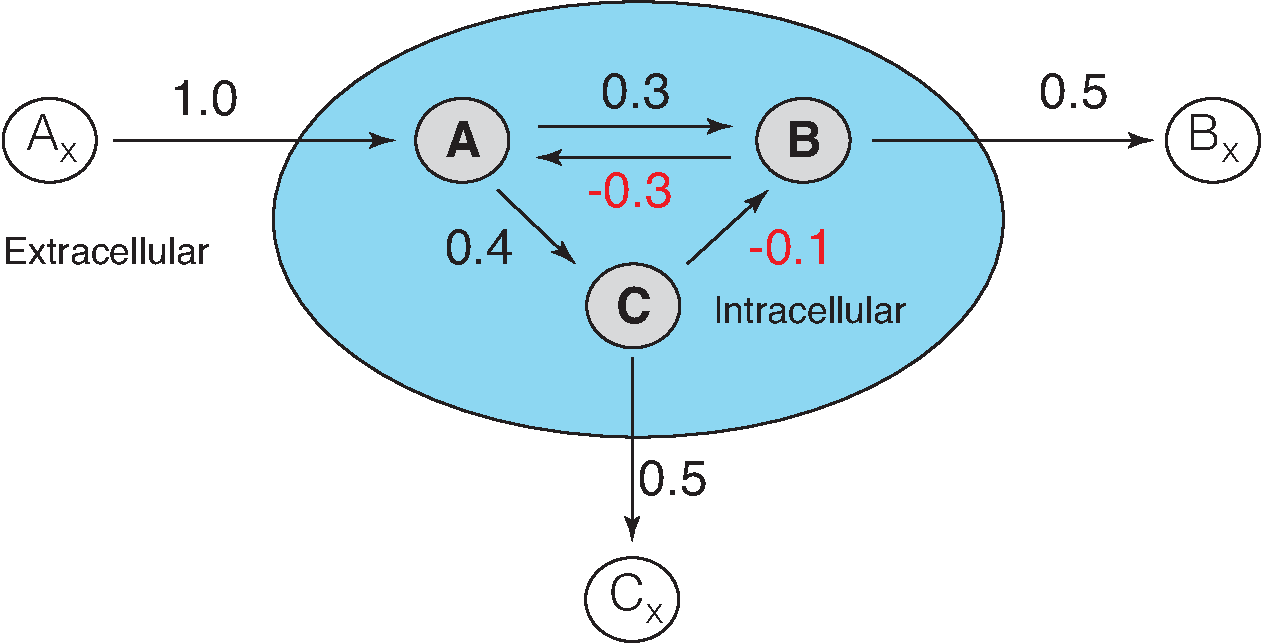
\psfig{file=figs/Simple-network-example-flux-solution-eps-converted-to.pdf,width=0.8\textwidth}
\caption{Example flux solution for $q_{1} = 1.0$ and $q_{2} = 0.5$.
While the overall material balance is consistent, some estimated intracellular fluxes ($v_{3}$ and $v_{4}$) violate non-negativity.}\label{fig-bad-flux-solution}
\end{figure*}

We can resolve the non-negativity issue by further constraining the relationships between the fluxes.
However, the formulation of these additional constraints are case specific. In the simplest case, let's assume there is no flux through $v_{4}$.
Thus, we move $v_{4}$ to the measured list and and redefine $\mathbf{\Sigma}$ and $\mathbf{\Phi}$ as:

\begin{equation}
\mathbf{\Sigma} =
\begin{bmatrix}
	-1 & -1 & 0 & 0 \\
	1 & 0 & 1 & 0 \\
	0 & 1 & -1 & -1 \\
\end{bmatrix}
\end{equation} and
\begin{equation}
	\mathbf{\Phi} =
	\begin{bmatrix}
		1 & 0 & 1 \\
		0 & -1 & -1 \\
		0 & 0 & 0 \\
	\end{bmatrix}
\end{equation}
The $rank\left(\mathbf{\Sigma}\right)$ = 3, and the solution (assuming $q_{1} = 1.0$, $q_{2} = 0.5$ and $v_{4} = 0.0$) is shown in Fig. \eqref{fig-bad-flux-solution-corrected}.

\begin{figure*}[h!]\centering
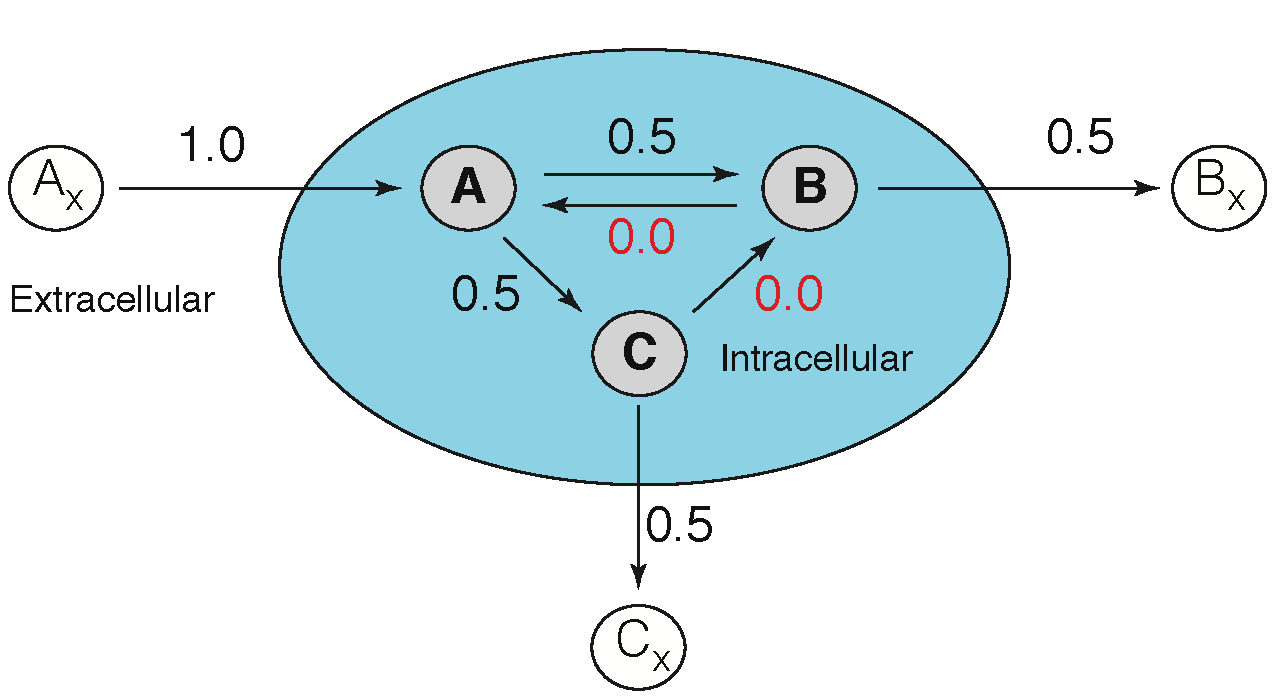
\psfig{file=figs/BadSolnCorrected-MFA.pdf,width=0.8\textwidth}
\caption{Example flux solution for $q_{1} = 1.0$, $q_{2} = 0.5$ and $v_{4} = 0.0$.
The overall material balance is consistent, and no intracellular fluxes violate non-negativity. However, we required an additional measurement (constraint) to calculate the solution}\label{fig-bad-flux-solution-corrected}
\end{figure*}

%\bibliography{Notes}
\end{document}
